\section{Solution}
In this section we describe the key ideas behind our design, and the decisions we made during the design process.

First we had to decide which design option of the 4 given options we were going to use. As seen in our answers to question 3 in section ~\ref{sec:Q3} a naive scaler is very inefficient, it is actually not possible to implement such a scaler on the Xilinx boards we use in the lab. So we will implement the scaler using the direct equation. Now we have to decide between doing the scaling directly, or composing it of multiple scalers. The trade-of here is that a direct scaler has to store more coefficients on the board, whereas a composed scaler uses more multiplications per output. Also, for each scaler we introduce in a composed scaler the delay of the system is increased. We decided to use one direct scaler from $44.1$ KHz to $48$ KHz.

The next choice we had to make was whether to optimize the scaler for resource usage or for throughput. We decided to optimize for throughput. The most important implication this choice has is that we will use 4 parallel multipliers for the FIR, instead of doing 4 sequential multiplications on one multiplier. We can now compose a diagram of the architecture of our system, figure ~\ref{fig:arch}. The coefficients are stored in read only memory (ROM), not visible in the diagram. Some additional hardware is required to get the right coefficient \texttt{h[i]} our of the ROM.

To generate the actual coefficients we wrote a small Java program that given some \texttt{L} spits out all coefficients  in 16 bit signed hex notation. We scaled the coefficients such that they sum up to $(2^{15}-1)\cdot 4 = 131068$, this way the output signal will have the same intensity as the input signal.

\begin{figure}
\begin{center}
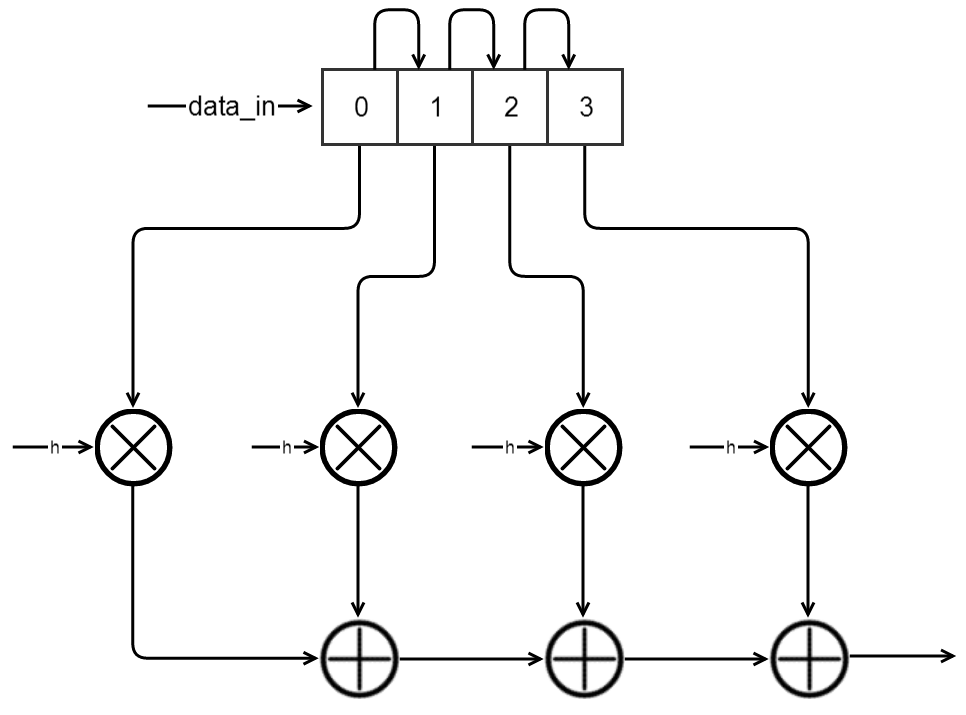
\includegraphics[width=0.7\textwidth]{images/architecture.png}
\caption{Architecture diagram of the scaler.}
\label{fig:arch}
\end{center}
\end{figure}

Another observation we made is that since the \texttt{lanczos} function is symmetric, the coefficients are symmetric as well. Therefore we could optimize our program by only storing half the coefficients, more precisely we only store $2L + 1$ coefficients instead of $4L$. After implementing this we noticed that as well as using less registers, the post PAR static timing report showed an increase in clock frequency. This can be explained by a more efficient routing because we use less wires.
